\section{Riemann and the Geometry of Space: From Decomposition to Curvature}

If Fourier showed that any vibration could be decomposed into waves,  
and Cayley showed that transformations could be encoded in algebra,  
then Bernhard Riemann asked a deeper, more radical question:

\begin{quote}
What if space itself is not fixed—but a flexible entity, whose very fabric can bend, stretch, and curve?
\end{quote}

Where Fourier decomposed functions into modes,  
and Cayley abstracted geometry into algebraic relations,  
Riemann synthesized these insights into a new vision:

Geometry is not just about figures drawn in space. Geometry is about the properties of space itself.

\subsection{The Leap from Fourier and Cayley to Riemann}

Cayley had turned geometric relationships into algebraic structures,  
introducing matrices, determinants, and invariants under transformation.

Fourier had shown that even the most complex phenomena could be decomposed into sums of simple oscillations.

Riemann saw that these transformations and decompositions were merely shadows of a deeper structure:  
the intrinsic geometry of a space, defined not by its embedding in a higher-dimensional Euclidean setting,  
but by quantities measured purely within the space itself.

In his 1854 habilitation lecture, Riemann proposed that the notions of distance, angle, and curvature  
did not need to come from Euclidean space at all.  
Instead, they could be defined at each point by a **metric tensor** \( g_{ij}(x) \)—  
a local rule for measuring lengths and angles infinitesimally.

\begin{HistoricalSidebar}{The Shift from Cayley and Fourier to Riemann}
In the mid-19th century, Arthur Cayley and Joseph Fourier reshaped geometry by showing how objects could be 
manipulated and decomposed within a fixed, underlying space.  Cayley introduced matrices and determinants to 
describe linear transformations—rotations, reflections, shears—and Fourier developed the idea of breaking 
complicated functions into simple sine and cosine “building blocks.”  Together, their work treated geometry 
and analysis as questions of how figures and signals change under explicit operations or basis‐function expansions.

\medskip

Bernhard Riemann’s breakthrough took an entirely different tack: he proposed that space itself has a 
geometry that can vary from point to point.  Instead of focusing on transformations of shapes embedded 
in an invisible Euclidean backdrop, Riemann endowed each infinitesimal neighborhood with its own metric 
tensor \(g_{ij}\), a smooth field prescribing distances and angles intrinsically.  In his view, geometry 
was not about moving rigid objects around but about the curvature and structure woven into the fabric of 
space itself.

\medskip

In other words, Cayley and Fourier gave us the algebra of transformations and the art of decomposing functions, 
while Riemann handed us the notion that space’s very geometry is dynamic—encoded in a tensor that tells us how 
to measure lengths and detect curvature at every point.  
\end{HistoricalSidebar}






\subsection{The Birth of Intrinsic Geometry}

With Riemann’s insight, geometry was freed from the tyranny of the flat plane.  No longer did we need to imagine that lines and distances were given “from above” by an ambient Euclidean world—instead, every notion of length and straightness sprang from the manifold itself.  At each point, a little “ruler” (the metric tensor \(g_{ij}\)) tells you exactly how to convert coordinate differences into physical distances; those rulers can vary from place to place, so that an infinitesimal step in one direction might be longer or shorter than the same coordinate step elsewhere.

Straight lines become \emph{geodesics}—the paths that locally minimize distance according to the metric.  On a gently rolling hill (a two‐dimensional example), the shortest route between two points may curve to follow the valley floor; on a sphere, “straight” great‐circle routes bend across the sky.  Because the metric can twist and stretch the fabric of space itself, there may be multiple inequivalent “shortest” paths between the same pair of points, or none at all if the space is too wildly contorted.

Curvature likewise ceases to be a curious ornament of curves in a plane and becomes a local property of the manifold.  Riemann showed how to compute at each point whether the space is “saddle‐shaped,” “spherical,” or “flat,” purely from derivatives of the metric tensor.  This intrinsic curvature dictates how triangles’ angles sum to more or less than \(180^\circ\), how parallel lines converge or diverge, and how volumes grow with radius in small balls.

Philosophically, this was a revolution: geometry no longer sits behind physics as a passive stage—it participates in the drama.  Matter and energy can tell the manifold how to curve, and that curvature back‐reacts on the motion of particles (as in Einstein’s general relativity).  In Riemann’s world, the shape of space is both the canvas and a character in the story of motion.

\begin{figure}[H]
    \centering
    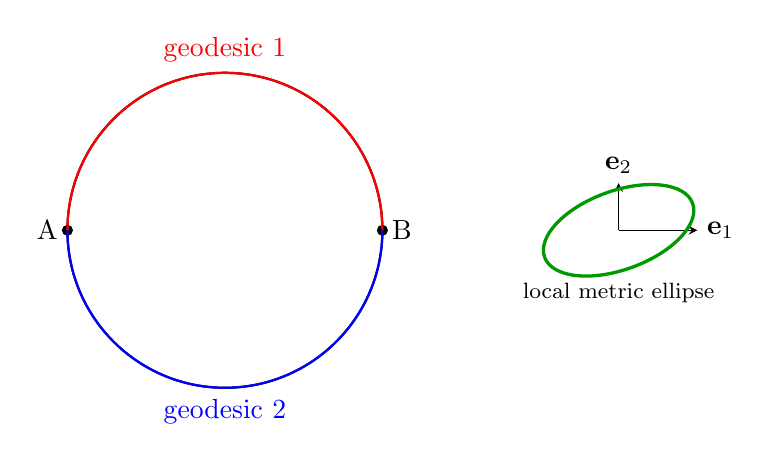
\begin{tikzpicture}[>=stealth,scale=1]
      % Sphere cross‐section
      \draw[thick] (0,0) circle (2cm);
      % Two antipodal points A and B
      \coordinate (A) at (-2,0);
      \coordinate (B) at (2,0);
      \fill (A) circle (2pt) node[left]  {A};
      \fill (B) circle (2pt) node[right] {B};
      % Two distinct geodesics (great‐circle arcs)
      \draw[red,thick]   (A) arc[start angle=180,end angle=0,radius=2cm];
      \draw[blue,thick]  (A) arc[start angle=180,end angle=360,radius=2cm];
      % Labels on arcs
      \node[red]  at (0, 2.3) {geodesic 1};
      \node[blue] at (0,-2.3) {geodesic 2};
      % Inset: local metric at a point
      \begin{scope}[xshift=5cm, yshift=0cm]
        % small coordinate patch
        \draw[->] (0,0) -- (1,0) node[right] {$\mathbf e_1$};
        \draw[->] (0,0) -- (0,0.6) node[above] {$\mathbf e_2$};
        % metric ellipse showing g_ij
        \draw[rotate=20,green!60!black,very thick] (0,0) ellipse (1cm and 0.5cm);
        \node at (0,-0.8) {\footnotesize local metric ellipse};
      \end{scope}
    \end{tikzpicture}
    \caption{%
    A cross‐section of a sphere: two antipodal points \(A\) and \(B\) are connected by infinitely many great‐circle geodesics; here two are shown in red and blue.  
    At right is a depiction of the local metric tensor \(g_{ij}\): its unit‐circle image (green ellipse) shows how “length” depends on direction in a curved manifold.}
\end{figure}


\begin{figure}[H]
    \centering
    \begin{tikzpicture}[>=stealth,scale=1]
      % Deformed coordinate grid
      \foreach \y in {0,1,2,3,4}{
        \draw[gray!50] plot[smooth] coordinates {(0,\y) (1,\y+0.2) (2,\y) (3,\y-0.2) (4,\y)};
      }
      \foreach \x in {0,1,2,3,4}{
        \draw[gray!50] plot[smooth] coordinates {(\x,0) (\x+0.2,1) (\x,2) (\x-0.2,3) (\x,4)};
      }
    
      % Points P and Q
      \filldraw[black] (0.5,0.5) circle (2pt) node[below left] {P};
      \filldraw[black] (3.5,3.5) circle (2pt) node[above right] {Q};
    
      % Geodesics
      \draw[red,thick,smooth]   plot coordinates {(0.5,0.5) (1,1) (2,1.8) (3,2.8) (3.5,3.5)};
      \draw[blue,thick,smooth]  plot coordinates {(0.5,0.5) (1.2,0.8) (2.2,1.8) (3,3) (3.5,3.5)};
    
      % Metric ellipses
      \draw[green!60!black,very thick,rotate around={-20:(1,1)}] (1,1) ellipse (0.3cm and 0.1cm);
      \draw[orange,very thick,rotate around={30:(2,2)}]        (2,2) ellipse (0.4cm and 0.2cm);
      \draw[purple,very thick,rotate around={60:(3,3)}]        (3,3) ellipse (0.2cm and 0.5cm);
    
      % Legend
      \node[draw, fill=white, inner sep=5pt] at (-3,4.3) {
        \begin{tikzpicture}[>=stealth,scale=0.8]
          \draw[gray!50] (0,0) -- (0.5,0) node[right]{coordinate grid};
          \draw[red,thick] (0,-0.3) -- (0.5,-0.3) node[right]{geodesic 1};
          \draw[blue,thick] (0,-0.6) -- (0.5,-0.6) node[right]{geodesic 2};
          \filldraw[black] (0,-0.9) circle (1.5pt) node[right]{points P, Q};
          \draw[green!60!black,very thick] (0,-1.2) ellipse (0.2cm and 0.1cm) node[right]{metric ellipse};
        \end{tikzpicture}
      };
    \end{tikzpicture}
    \caption{%
    A patch of a Riemannian manifold illustrated by a deformed coordinate grid.  
    Points \(P\) and \(Q\) (black dots) are connected by two distinct geodesics (red, blue).  
    Local metric tensors \(g_{ij}\) are depicted by ellipses (green, orange, purple) showing directional scaling.}
\end{figure}
    

\begin{HistoricalSidebar}{The Parallel Postulate and the Seeds of Curvature}

  For over two millennia, Euclid's parallel postulate stood apart—an axiom that seemed clumsy, arbitrary, 
  and possibly unnecessary. Generations of mathematicians attempted to derive it from the others, hoping to banish 
  its awkwardness. But in the early 19th century, a radical shift occurred: rather than proving the parallel 
  postulate, figures like Gauss, Lobachevsky, and Bolyai constructed entire geometries where it simply failed 
  to hold. In these non-Euclidean spaces, the sum of a triangle’s angles could be less than \(180^\circ\), and 
  multiple lines could run through a point without ever intersecting a given line.

  \medskip
  
  The existence of multiple valid geometries shattered the old certainty that Euclidean space was the only possible 
  geometry. If space could bend, how should one even define geometry itself? Was there a deeper, more universal 
  language that could describe Euclidean and non-Euclidean worlds as special cases of a larger framework?

  \medskip
  
  This was the atmosphere into which Bernhard Riemann stepped. Unlike his predecessors, he was not content to 
  merely classify geometries by how many parallels exist; instead, he asked how one could describe the 
  \textbf{shape of space} intrinsically, at each infinitesimal point, without reference to any external embedding. 
  His introduction of the metric tensor \(g_{ij}\) provided precisely that tool: a local formula for distance, 
  encoding how space might bend, twist, or flatten from place to place.

  \medskip
  
  Where Lobachevsky and Bolyai discovered that Euclid’s fifth postulate was not unique, Riemann dissolved the 
  entire debate by showing that "geometry" itself was far broader than anyone had imagined: it was a continuous 
  spectrum, with curvature as its master parameter.
\end{HistoricalSidebar}

    




\subsection{From Curves to Curvature}

Riemann’s great leap was to recognize that a manifold can bend and twist in infinitely many ways, and that this local deformation is captured by a single multi–index object: the \emph{curvature tensor} \(R^i{}_{jkl}\).  Rather than merely recording how a linear map stretches or rotates vectors (as Cayley’s matrices do), the curvature tensor measures how a vector is “mismatched” with itself after being carried around an infinitesimal loop.  If the manifold were truly flat, that loop would close perfectly; if not, the failure to return to the original direction quantifies the intrinsic curvature in each pair of directions.

In Fourier’s world, one decomposes a function into sines and cosines—global modes that live on a fixed background.  Riemann turned that idea inside out: he showed that the “background” of space itself can vary from point to point.  Each infinitesimal neighborhood looks like ordinary Euclidean space, but the way these patches are glued together is governed by the curvature tensor.  In this sense, Riemann “decomposed” geometry into a continuum of local Euclidean pieces, stitched by curvature data, rather than decomposing functions into global harmonic modes.

\begin{itemize}
    \item Euler formulated motion in terms of forces, 
    \begin{itemize}
        \item but those vector‐based equations became unwieldy for complex systems
    \end{itemize}
    \item therefore Lagrange recast dynamics as the problem of extremizing an action
    \begin{itemize}
        \item but the action principle still masked the underlying geometric structure
    \end{itemize}
    \item therefore Hamilton revealed that trajectories are flows in a higher-dimensional phase space
    \begin{itemize}
        \item but integrating many such flows remained cumbersome
    \end{itemize}
    \item therefore Jacobi showed that all these flows arise as normals to the level‐set surfaces of a single function \(S\), 
    \begin{itemize}
        \item but this picture still relied on a fixed backdrop
    \end{itemize}
    \item therefore Cayley abstracted geometry into the algebra of matrices and determinants, 
    \begin{itemize}
        \item but his linear‐algebraic tools did not address the global decomposition of functions
    \end{itemize}
    \item therefore Fourier taught us to decompose complex vibrations into simple sine and cosine modes, 
    \begin{itemize}
        \item but space itself remained undeformed
    \end{itemize}
    \item therefore Riemann liberated geometry from its Euclidean constraints by introducing a point-wise metric tensor, thus making the shape of space itself the fundamental actor in the drama of physics.  
\end{itemize}



\subsection{A Glimpse at Riemann’s Curvature without Christoffel Symbols}

Riemann defined curvature intrinsically by examining how the metric coefficients \(g_{ij}(x)\) deviate from the flat‐space form when expanded about a point.  His approach—even before the later notation of Christoffel symbols—proceeds in three steps:

\textbf{1. The line element.}  On an \(n\)–dimensional manifold with local coordinates \(x^1,\dots,x^n\), the squared distance is
\[
ds^2 \;=\; \sum_{i,j=1}^n g_{ij}(x)\,dx^i\,dx^j.
\]


\begin{figure}[H]
    \centering
    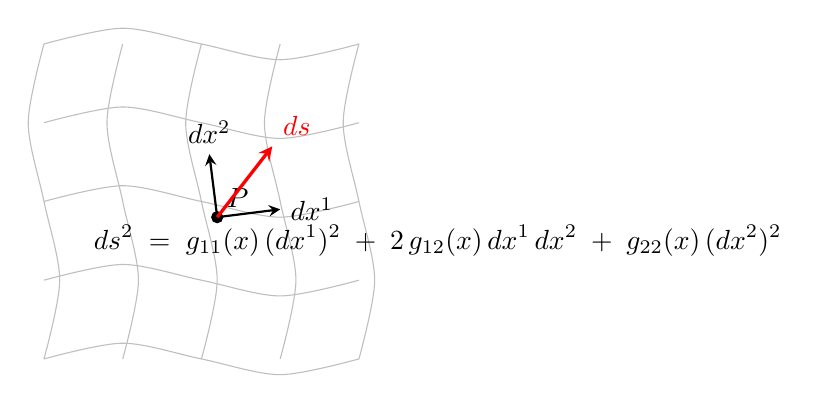
\begin{tikzpicture}[>=stealth,scale=1]
      % Deformed coordinate grid (manifold patch)
      \foreach \y in {0,1,2,3,4}{
        \draw[gray!50] plot[smooth] coordinates {(0,\y) (1,\y+0.2) (2,\y) (3,\y-0.2) (4,\y)};
      }
      \foreach \x in {0,1,2,3,4}{
        \draw[gray!50] plot[smooth] coordinates {(\x,0) (\x+0.2,1) (\x,2) (\x-0.2,3) (\x,4)};
      }
    
      % Point P
      \coordinate (P) at (2.2,1.8);
      \filldraw[black] (P) circle (2pt) node[above right] {$P$};
    
      % Differential coordinate vectors dx^1 and dx^2
      \draw[->,thick] (P) -- ++(0.8,0.1) node[right] {$dx^1$};
      \draw[->,thick] (P) -- ++(-0.1,0.8) node[above] {$dx^2$};
    
      % Resultant displacement vector ds
      \draw[->,red,very thick] 
        (P) -- ++(0.7,0.9) node[above right] {$ds$};
    
      % Formula for the line element
      \node at (5,1.5) {\(\displaystyle 
        ds^2 \;=\; g_{11}(x)\,(dx^1)^2 
        \;+\;2\,g_{12}(x)\,dx^1\,dx^2 
        \;+\;g_{22}(x)\,(dx^2)^2
        \)};
    \end{tikzpicture}
    \caption{%
    Illustration of the line element on a 2D manifold: at point \(P\) in local coordinates \((x^1,x^2)\), 
    the small coordinate displacements \(dx^1\) and \(dx^2\) combine to produce the infinitesimal distance \(ds\).  
    The metric coefficients \(g_{ij}(x)\) weight each term in the expression \(ds^2 = g_{ij}\,dx^i\,dx^j\).}
\end{figure}


\textbf{2. Geodesic (normal) coordinates.}  One picks coordinates centered at a point \(p\) so that at \(p\),
\[
g_{ij}(p) \;=\;\delta_{ij},
\qquad
\frac{\partial g_{ij}}{\partial x^k}\Bigl|_{p} \;=\;0.
\]
In these “flat‐to‐first‐order” coordinates, the metric expands as
\[
g_{ij}(x)
\;=\;
\delta_{ij}
\;+\;
\frac12
\sum_{k,\ell=1}^n
\frac{\partial^2 g_{ij}}{\partial x^k\,\partial x^\ell}\Bigl|_{p}
\,x^k\,x^\ell
\;+\;
O(\|x\|^3).
\]


\begin{figure}[H]
    \centering
    \begin{tikzpicture}[>=stealth,scale=1]
      % Deformed background grid (manifold patch)
      \foreach \y in {0,1,2,3,4}{
        \draw[gray!50] plot[smooth] coordinates {
          (0,\y) (1,\y+0.2) (2,\y+0.3) (3,\y+0.2) (4,\y)
        };
      }
      \foreach \x in {0,1,2,3,4}{
        \draw[gray!50] plot[smooth] coordinates {
          (\x,0) (\x+0.2,1) (\x+0.3,2) (\x+0.2,3) (\x,4)
        };
      }
    
      % Point p
      \coordinate (p) at (2,2);
      \filldraw[black] (p) circle (2pt) node[above right] {$p$};
    
      % Tangent (normal) coordinates at p: orthonormal basis
      \draw[->,blue,very thick] (p) -- ++(0.8,0) node[right] {$\mathbf e_1$};
      \draw[->,blue,very thick] (p) -- ++(0,0.8) node[above]   {$\mathbf e_2$};
    
      % Unit circle in these coordinates: g_ij(p)=delta_ij
      \draw[blue,thick] (p) circle (0.5cm);
      \node[blue] at ($(p)+(1.1,0.6)$) {\small $g_{ij}(p)=\delta_{ij}$};
    
      % Indicate vanishing first derivatives ∂g|_p = 0
      \draw[<->,black] ($(p)+(-0.4,0.7)$) -- node[left]{\small $\partial_k g_{ij}|_p=0$} ($(p)+(-0.4,0.3)$);
    
      % Curvature from second derivatives: grid bending
      \node at (3.5,1) {\small curvature from $\partial^2 g_{ij}$};
    
    \end{tikzpicture}
    \caption{%
    In normal (geodesic) coordinates around \(p\), the metric at \(p\) reduces to the identity (\(g_{ij}(p)=\delta_{ij}\)) and its first derivatives vanish (\(\partial_k g_{ij}|_p=0\)), so infinitesimal distances there behave like flat space (blue unit circle).  Further out, the slight bending of the grid illustrates the second‐order terms \(\tfrac12\,\partial_k\partial_\ell g_{ij}|_p\,x^k x^\ell\) in the expansion of \(g_{ij}(x)\).}
\end{figure}




\textbf{3. Curvature coefficients.}  
Riemann then defined the components of the curvature tensor by combining these second derivatives:
\[
R_{i k \ell j}(p)
\;=\;
\frac12\Bigl(
\underbrace{\partial_k\partial_\ell\,g_{ij}}_{A}
\;-\;
\underbrace{\partial_k\partial_j\,g_{i\ell}}_{B}
\;-\;
\underbrace{\partial_i\partial_\ell\,g_{kj}}_{C}
\;+\;
\underbrace{\partial_i\partial_j\,g_{k\ell}}_{D}
\Bigr)_{\!p}.
\]
If the space were flat, all second derivatives would vanish and hence \(R_{i k \ell j}=0\).  Nonzero components measure the “bending” of the manifold in the planes spanned by the coordinate directions \(i,k\) (and similarly \(j,\ell\)).


\begin{figure}[H]
    \centering
    \begin{tikzpicture}[scale=1]
      % Macro to draw a curved grid patch at (x,y) with bulge amount b
      \newcommand{\drawpatch}[3]{%
        \begin{scope}[shift={({#1},{#2})}]
          \foreach \yy in {0.2,0.6,1.0}{
            \draw[gray!50] plot[smooth] coordinates {(0,\yy) (0.5,\yy+#3) (1,\yy)};
          }
          \foreach \xx in {0.2,0.6,1.0}{
            \draw[gray!50] plot[smooth] coordinates {(\xx,0) (\xx+#3,0.5) (\xx,1)};
          }
        \end{scope}%
      }
    
      % Four patches with different curvature signs
      \drawpatch{-1}{1}{0.1}   % A
      \drawpatch{1}{1}{-0.1}   % B
      \drawpatch{-1}{-1}{0.2}  % C
      \drawpatch{1}{-1}{-0.2}  % D
    
      % Labels for each patch
      \node at (-1,1.8)  {\textbf{A}};
      \node at (1,1.8)   {\textbf{B}};
      \node at (-1,-0.2) {\textbf{C}};
      \node at (1,-0.2)  {\textbf{D}};
    
      % Curvature formula beneath
      \node at (0,-2.2) {\(\displaystyle
        R_{i k \ell j}(p)
        \;=\;\tfrac12\bigl(
          \partial_k\partial_\ell\,g_{ij}
        \;-\;\partial_k\partial_j\,g_{i\ell}
        \;-\;\partial_i\partial_\ell\,g_{kj}
        \;+\;\partial_i\partial_j\,g_{k\ell}
        \bigr)_{\!p}.
      \)};
    \end{tikzpicture}
    \caption{%
    Four infinitesimal patches (A–D) of a curved manifold exhibit different “bulges” in their coordinate grids, corresponding to the second derivatives of the metric in various directions.  Riemann’s curvature coefficient \(R_{i k \ell j}(p)\) at point \(p\) is built by combining these four second‐derivative patterns.}
    \end{figure}
    







\textbf{Two‐dimensional case.}  In two dimensions there is only one independent curvature component, often called the Gaussian curvature \(K\).  One finds
\[
K(p)
\;=\;
\frac{R_{1 2 2 1}(p)}{\det\bigl[g_{ij}(p)\bigr]}\,,
\]
so that \(K>0\) describes a locally spherical “hill,” \(K<0\) a saddle shape, and \(K=0\) a flat plane.

\medskip
Thus, by expanding the metric in special coordinates and inspecting its second‐order terms, Riemann extracted an intrinsic measure of curvature—without ever invoking Christoffel symbols—revealing how space itself can bend and twist.  



\begin{figure}[H]
    \centering
    \begin{tikzpicture}[>=stealth,scale=1]
    
      % Macro: draw a 2×2 grid patch at horizontal shift #1,
      % with horizontal bulge #2 and vertical bulge #3, label #4.
      \newcommand{\gridpatch}[4]{%
        \begin{scope}[xshift=#1]
          % horizontal grid lines
          \foreach \y in {0,0.5,1,1.5,2}{
            \draw[gray!50] plot[smooth] coordinates {(0,\y) (1,\y + #2) (2,\y)};
          }
          % vertical grid lines
          \foreach \x in {0,0.5,1,1.5,2}{
            \draw[gray!50] plot[smooth] coordinates {(\x,0) (\x,1 + #3) (\x,2)};
          }
          % curvature label
          \node at (1,-0.3) {\small #4};
        \end{scope}%
      }
    
      % Hill (Gaussian curvature > 0)
      \gridpatch{-4cm}{0.3}{0.3}{$K>0$}
    
      % Flat plane (Gaussian curvature = 0)
      \gridpatch{0cm}{0}{0}{$K=0$}
    
      % Saddle (Gaussian curvature < 0)
      \gridpatch{4cm}{0.3}{-0.3}{$K<0$}
    
      % Axes labels
      \foreach \X in {-4,0,4}{
        \node at (\X,2.3) {\small local patch};
        \draw[->] (\X,0) -- ++(2.2,0) node[right] {$x^1$};
        \draw[->] (\X,0) -- ++(0,2.2) node[above] {$x^2$};
      }
    
    \end{tikzpicture}
    \caption{%
    Three infinitesimal 2D patches illustrating Gaussian curvature \(K\):
    \emph{left:} \(K>0\) (hill‐shaped), 
    \emph{center:} \(K=0\) (flat), 
    \emph{right:} \(K<0\) (saddle‐shaped).}
\end{figure}







\subsection{Reinterpreting Kepler’s Second Law in Riemann’s Own Language}

Kepler’s observation—that a planet sweeps out equal areas in equal times—can be seen not as a quirk of flat‐plane geometry but as a direct consequence of the circular symmetry of the space around a central mass.

Consider the two‐dimensional “orbital” manifold with line element, in polar‐type coordinates \((r,\theta)\),
\[
ds^2 \;=\; dr^2 \;+\; g_{\theta\theta}(r)\,d\theta^2,
\]
where in ordinary Euclidean space \(g_{\theta\theta}(r)=r^2\), while in the presence of a mass the function \(g_{\theta\theta}(r)\) may be slightly deformed.  Crucially, the metric coefficients depend only on \(r\), never on \(\theta\):
\[
\frac{\partial g_{ij}}{\partial \theta} \;=\; 0.
\]
Such a “cyclic” coordinate implies that along any geodesic the quantity
\[
p_\theta
\;=\;
g_{\theta\theta}(r)\,\frac{d\theta}{ds}
\]
remains constant.  Converting from arc‐length \(s\) to physical time \(t\) then gives
\[
g_{\theta\theta}(r)\,\frac{d\theta}{dt}
\;=\;
\text{constant}
\quad\Longrightarrow\quad
\tfrac12\,g_{\theta\theta}(r)\,\dot\theta
\;=\;
\frac{dA}{dt}
\;=\;
\text{constant}.
\]
In other words, because the line element does not “notice” any change in \(\theta\), the combination \(g_{\theta\theta}(r)\,\dot\theta\) is fixed along the path.  But \(g_{\theta\theta}(r)\,\dot\theta\) is exactly twice the areal velocity \(dA/dt\).  Thus the equal‐area law is built into the very shape of the manifold: the geodesic motion in a radially symmetric metric sweeps out equal areas in equal times by construction.

\begin{quote}
Kepler saw a sweep.  
Riemann saw a manifold whose rotational symmetry made it inevitable.
\end{quote}



\begin{figure}[H]
    \centering
    \begin{tikzpicture}[>=stealth,scale=1]
      % 1) Curved grid patch
      \foreach \y in {-1.5,-0.5,0.5,1.5}{
        \draw[gray!50] plot[smooth] coordinates {(-2,\y) (0,{\y+0.5}) (2,\y)};
      }
      \foreach \x in {-2,-1,1,2}{
        \draw[gray!50] plot[smooth] coordinates {(\x,-1.5) ({\x+0.5},0) (\x,1.5)};
      }
    
      % 2) Elliptical geodesic: r = a(1−e²)/(1+e cos θ), a=2, e=0.5
      \draw[blue,thick,domain=0:360,samples=200,smooth]
        plot ({(2*(1-0.5^2)/(1+0.5*cos(\x)))*cos(\x)},
             {(2*(1-0.5^2)/(1+0.5*cos(\x)))*sin(\x)});
    
      % 3) Two equal-area wedges along the ellipse
      \pgfmathsetmacro{\thetaA}{30}
      \pgfmathsetmacro{\thetaB}{120}
      \pgfmathsetmacro{\rA}{2*(1-0.5^2)/(1+0.5*cos(\thetaA))}
      \pgfmathsetmacro{\rB}{2*(1-0.5^2)/(1+0.5*cos(\thetaB))}
      \pgfmathsetmacro{\dT}{0.6}
    
      % First wedge
      \coordinate (W1a) at ({\rA*cos(\thetaA+0.3)},{\rA*sin(\thetaA+0.3)});
      \coordinate (W1b) at ({\rA*cos(\thetaA-0.3)},{\rA*sin(\thetaA-0.3)});
      \fill[blue!20]
        (0,0) -- (W1b)
        arc[start angle={\thetaA-0.3}, end angle={\thetaA+0.3}, radius=\rA]
        -- cycle;
      \node[blue] at ({\rA*cos(\thetaA)},{\rA*sin(\thetaA)+0.3}) {$\Delta\theta_1$};
    
      % Second wedge
      \coordinate (W2a) at ({\rB*cos(\thetaB+0.2)},{\rB*sin(\thetaB+0.2)});
      \coordinate (W2b) at ({\rB*cos(\thetaB-0.2)},{\rB*sin(\thetaB-0.2)});
      \fill[green!20]
        (0,0) -- (W2b)
        arc[start angle={\thetaB-0.2}, end angle={\thetaB+0.2}, radius=\rB]
        -- cycle;
      \node[green!60!black] at ({\rB*cos(\thetaB)},{\rB*sin(\thetaB)+0.3}) {$\Delta\theta_2$};
    
      % Legend
      \node[draw,fill=white,inner sep=6pt] at (-6,2.5) {
        \begin{tikzpicture}[>=stealth,scale=0.8]
          \draw[gray!50] (0,0) -- (0.6,0) node[right]{metric coordinate lines};
          \draw[blue,thick] (0,-0.4) -- (0.6,-0.4) node[right]{geodesic (orbit)};
          \fill[blue!20] (0,-0.8) rectangle (0.6,-1.0) node[right]{wedge at $r_1$};
          \fill[green!20] (0,-1.2) rectangle (0.6,-1.4) node[right]{wedge at $r_2$};
        \end{tikzpicture}
      };
    \end{tikzpicture}
    \caption{%
    On a radially symmetric manifold with line element $ds^2 = dr^2 + g_{\theta\theta}(r)\,d\theta^2$, two infinitesimal wedges at radii $r_1<r_2$ are chosen so that $g_{\theta\theta}(r_1)\,\Delta\theta_1 = g_{\theta\theta}(r_2)\,\Delta\theta_2$, making their intrinsic areas equal. This demonstrates that a geodesic in such a metric sweeps out equal areas in equal angular intervals purely by virtue of the manifold’s rotational symmetry.}
\end{figure}
    
    
    








\begin{figure}[H]
    \centering
    \begin{tikzpicture}[>=stealth,scale=1]
      % 1) Curved grid patch
      \foreach \y in {-1.5,-0.5,0.5,1.5}{
        \draw[gray!50] plot[smooth] coordinates {(-2,\y) (0,{\y+0.5}) (2,\y)};
      }
      \foreach \x in {-2,-1,1,2}{
        \draw[gray!50] plot[smooth] coordinates {(\x,-1.5) ({\x+0.5},0) (\x,1.5)};
      }
    
      % 2) Elliptical geodesic: r = a(1-e^2)/(1+e cos θ), a=2, e=0.5
      \draw[blue,thick,domain=0:360,samples=200,smooth]
        plot ({(2*(1-0.5^2)/(1+0.5*cos(\x)))*cos(\x)},
             {(2*(1-0.5^2)/(1+0.5*cos(\x)))*sin(\x)});
    
      % 3) Two equal-area parallelograms along the ellipse
      \pgfmathsetmacro{\thetaA}{30}
      \pgfmathsetmacro{\thetaB}{120}
      \pgfmathsetmacro{\rA}{2*(1-0.5^2)/(1+0.5*cos(\thetaA))}
      \pgfmathsetmacro{\rB}{2*(1-0.5^2)/(1+0.5*cos(\thetaB))}
      \pgfmathsetmacro{\dR}{0.25}
      \pgfmathsetmacro{\dT}{0.45}
    
      \coordinate (P1) at ({\rA*cos(\thetaA)},{\rA*sin(\thetaA)});
      \coordinate (dR1) at ({\dR*cos(\thetaA)},{\dR*sin(\thetaA)});
      \coordinate (t1)  at ({-\dT*sin(\thetaA)},{\dT*cos(\thetaA)});
    
      \coordinate (P2) at ({\rB*cos(\thetaB)},{\rB*sin(\thetaB)});
      \coordinate (dR2) at ({\dR*cos(\thetaB)},{\dR*sin(\thetaB)});
      \coordinate (t2)  at ({-\dT*sin(\thetaB)},{\dT*cos(\thetaB)});
    
      \fill[blue!20]
        (P1) -- ($(P1)+(dR1)$) -- ($(P1)+(dR1)+(t1)$) -- ($(P1)+(t1)$) -- cycle;
      \fill[blue!20]
        (P2) -- ($(P2)+(dR2)$) -- ($(P2)+(dR2)+(t2)$) -- ($(P2)+(t2)$) -- cycle;
    
      % 4) Killing vector field arrow (rotation generator)
      \draw[orange,very thick,->] (2.3,0) arc[start angle=0,end angle=60,radius=2.3]
        node[midway,right] {\(\xi\)};
    
      % Legend with increased spacing
      \node[draw,fill=white,inner sep=6pt] at (-6,2.5) {
        \begin{tikzpicture}[>=stealth,scale=0.8]
          \matrix[row sep=0.5cm,ampersand replacement=\&]{
            \draw[gray!50] (0,0) -- (0.6,0);            \& \node{curved grid};     \\
            \draw[blue,thick] (0,0) -- (0.6,0);          \& \node{geodesic (orbit)};\\
            \fill[blue!20] (0,0) rectangle (0.6,-0.2);   \& \node{equal‐area};      \\
            \draw[orange,very thick,->] (0,0) -- (0.6,0);\& \node{Killing vector};   \\
          };
        \end{tikzpicture}
      };
    
    \end{tikzpicture}
    \caption{%
    A Riemannian reinterpretation of Kepler’s Second Law.  
    The gray curved grid shows the distorted coordinate patch (manifold).  
    The blue curve is the planet’s geodesic (elliptical orbit).  
    Two shaded parallelograms have equal intrinsic area \(\tfrac12\,r^2\,\Delta\theta\).  
    The orange arrow \(\xi\) is the rotation‐generating Killing vector, whose symmetry preserves area elements along the orbit.}
\end{figure}
    